\chapter{Approximate Inference for Stochastic Epidemic Models of Outbreaks in Large Populations}
\label{chap:lna_for_sems}

\section{Overview}
\label{sec:lna_overview}

Surveillance and outbreak response systems often report incidence counts of new cases detected in each inter--observation time interval. Analyzing this type of time series data is challenging since we must overcome many of the same challenges that we face in modeling the transmission dynamics of infectious diseases in small population settings with prevalence data --- discrete snapshots of a continuously evolving epidemic process, detecting a fraction of the new cases, and often directly observing only one aspect of the disease process. Furthermore, our task is made more difficult by the additional computational burden that results from repeated evaluation of CTMC likelihoods; the products of exponential waiting time distributions consist of polynomially increasing numbers of terms, and agent--based data augmentation (DA) MCMC algorithms become unwieldy as the numbers of subject--path proposals required to meaningfully perturb the CTMC likelihood get large \citep{fintzi2017efficient}. 

In this chapter, we show how the LNA of Section \ref{subsubsec:lna_background} can be adapted to obtain approximate inference for SEMs fit to epidemic count data in large populations. Our contributions are threefold: First, we demonstrate how the SEM dynamics should be reparameterized so that the LNA can be used to approximate transition densities of the counting processes for disease state transition events. Second, we fold the LNA into a Bayesian DA framework in which latent LNA paths are sampled using the elliptical slice sampling (EliptSS) algorithm of \cite{murray2010}. This provides us with general machinery for jointly updating the latent paths while absolving us of the \textit{de facto} modeling choice that the data be Gaussian in order to efficiently perform inference as in \cite{fearnhead2014,komorowski2009}, or the need to use computationally intensive particle filter methods for non--Gaussian emission distributions as in \cite{golightly2015delayed}. Finally, we introduce a non--centered parameterization (NCP) for the LNA that massively improves the efficiency of our DA MCMC framework and makes it tractable for fitting complex models. 

\section{Fitting Stochastic Epidemic Models via the Linear Noise Approximation}
\label{sec:lna_methods}

For clarity, we will present the algorithm for fitting SEMs via the LNA in the context of fitting the susceptible--infected--recovered (SIR) model to negative binomial distributed incidence counts. We will, however, provide notation where appropriate so that the generality of the algorithm should be apparent. The SIR model is an abstraction of the transmission dynamics of an outbreak as a closed, homogeneously mixing population of $ N $ exchangeable individuals who are either susceptible $ (S) $, infected, and hence infectious, $ (I) $, or recovered $ (R) $. It is important to note that the model compartments refer to disease states as they relate to the transmission dynamics, not the disease process. Thus, an individual is considered to be recovered when she no longer has infectious contact with other individuals in the population, not when she clears disease carriage. As another example, in the susceptible--exposed--infected--recovered (SEIR) type models that we will consider later, the latent period in which an individual is exposed, but not yet infectious, should be understood as possibly varying in population with different contact dynamics, even when the incubation period of the pathogen should arguably be consistent across groups.

\subsection{Measurement Process and Data}
\label{subsec:lna_measproc}
Incidence data, $ \bY = \lbrace Y_1,\dots,Y_L\rbrace $,  arise as increments of the numbers of new cases accumulated in a set of time intervals, $ \mcI = \lbrace\mcI_1,\dots,\mcI_L:\ \mcI_\ell = (t_{\ell-1},t_\ell]\rbrace $. In outbreak or surveillance settings, we do not typically believe that every case is detected since individuals may be asymptomatic or may escape detection. Let $ \bN^c = (N^c_{SI}, N^c_{IR}) $ denote the counting process for the cumulative numbers of infections ($ S\rightarrow I $ transitions) and recoveries ($ I\rightarrow R $ transitions), and let $ \Delta \bN^c(t_\ell) = \bN^c(t_\ell) - \bN^c(t_{\ell-1})$ denote the change in cumulative numbers of transitions over $ \mcI_\ell $; so, $ \Delta N^c_{SI}(t_\ell)$ is the incidence over $ (t_{\ell-1},t_\ell] $. We might choose to model the number of observed cases as a negative binomial sample of the true incidence with detection rate $ \rho $ and over--dispersion parameter $ \phi $. Thus,
\begin{equation}
\label{eqn:incidence_emitprob}
Y_\ell|\Delta N^c_{SI}(t_\ell),\rho \sim \mr{Neg.Binom.}(\mr{\mu} = \rho\Delta N^c_{SI}(t_\ell),\ \sigma^2 = \mu + \mu^2/\phi).
\end{equation}

There are two minor points that we wish to make note of before proceeding. First, we have allowed for the possibility that cases are over--reported. This is neither a necessary assumption for any of the subsequent results, nor is it unreasonable when studying outbreaks in large populations where the ``fog of war" might lead to inflation of reported incidence or misclassification of individuals whose symptoms are similar to the disease of interest. This modeling choice is also not particularly problematic when the detection probability is low since the emission densities will have negligible mass above the true incidence. Second, we are also making this modeling choice with an eye on the compatibility of the measurement distribution with the eventual LNA approximation, which takes real, not integer, values. The negative binomial distribution is well defined for non--integer values of the mean parameter. 

\subsection{Latent Epidemic Process}
\label{subsec:lna_epid_proc}

The SIR model is typically expressed in terms of compartment counts, $ \bX^c = \lbrace S^c,I^c,R^c\rbrace $, that evolve in continuous time on state space $ \mcS_X^c = \left \lbrace \mcC_{lmn}:l,m,n\in\lbrace0,\dots,N\rbrace,\ l+m+n=P\right \rbrace $. We will make the (not particularly limiting) modeling choice to express the waiting times between disease state transitions as being exponentially distributed. Thus, $ \bX $ evolves according to a Markov jump process (MJP). If our data had consisted of prevalence counts, which arise as partial observations of infected individuals, we might have chosen to approximate transition densities of the MJP for $ \bX $ in the usual way that appears in \cite{komorowski2009,fearnhead2014}. 

However, incidence data are discretely observed, partial realizations of the increments of counting processes that evolve continuously in time as individuals transition among disease states. The emission probabilities for incidence data, e.g., (\ref{eqn:incidence_emitprob}), depend on the change in $ N_{SI}^c $ over the time interval $ (t_{\ell-1},t_\ell] $, not on the change in $ I $ over the interval. It would be incorrect to treat incidence as simply the difference in prevalence. We could easily construct a scenario where there are positive numbers of infections, but where the prevalence does not change due to an equal number of recoveries. We need to construct the LNA that approximates transition densities of $ \bN $ if we are to write down correctly specified emission probabilities.

The cumulative incidence process for infections and recoveries, $ \bN^c $, is a Markov jump process state space $ \mcS_N^c = \left \lbrace \mcC_{jk}:j,k\in\lbrace0,\dots,N\rbrace\right \rbrace $. Let $ \beta $ denote the per--contact infection rate, and $ \mu $ denote the rate at which each infected individual recovers. The rate at which $ \bN^c $ transitions from state $ \bn $ to $ \bn^{\prime}$ is 
\begin{equation}
	\label{eqn:lna_sir_rates}
	\blambda_{\bn,\bn^\prime} = \left \lbrace \begin{array}{ll}
	\lambda_{SI} = \beta S I, & \bn = (n_{SI},n_{IR}),\ \bn^\prime = (n_{SI}+1,n_{IR}),\text{ and } n_{SI}+1\leq P, \\
	 \lambda_{IR} = \mu I, &  \bn = (n_{SI},n_{IR}),\  \bn^\prime = (n_{SI},n_{IR}+1),\text{ and } n_{IR}+1\leq P, \\
	 0, & \text{for all other } \bn \text{ and } \bn^\prime.
	\end{array} \right.
\end{equation}

\subsection{Tractable Approximations for Intractable Likelihoods}
\label{subsec:lna_motivation}
We would like to make inferences about the posterior distribution of the parameters, e.g., $ \btheta = (\beta, \mu, \bX(t_0), \rho)$, that govern the latent epidemic process and sampling distribution, 
\begin{align}
\label{eqn:intractable_posterior}
 \pi(\btheta|\bY)&\propto \pi(\bY|\btheta)\pi(\btheta) = \int L(\bY|\bN^c,\btheta)\pi(\bN^c|\btheta)\pi(\btheta)\rmd\pi(\bN^c)\nonumber\\
 &= \int_{\mcS^c}\prod_{\ell=1}^L \Pr\left (\bY_\ell|\Delta\bN_{SI}^c(t_\ell),\btheta\right )\pi\left (\bN^c(t_\ell)|\bn^c(t_{\ell-1}),\btheta\right )\pi(\btheta)\rmd\pi(\bN^c)
\end{align}
where $ \pi(\btheta) $ specifies the prior density of the model parameters. However, this integral is analytically intractable and is challenging to compute numerically due to the size of the state space of $ \bN^c $. In the following subsections, we will obtain the LNA for transition densities of $ \bN^c $, turning (\ref{eqn:intractable_posterior}) into an integral over a much more computationally tractable product of Gaussian densities and non--Gaussian emission probabilities. As we shall see, approximating the complete data likelihood in the posterior $ \pi(\btheta,\bN^c|\btheta) $ with a Gaussian state space model will open the doors to efficient algorithms for sampling from the approximate posterior. 

\subsection{Diffusion Approximation}
\label{subsec:diff_approx}

As outlined in Section \ref{subsubsec:diff_approx}, there are a variety of methods for arriving at a diffusion approximation for a Markov jump process, which under certain conditions yield equivalent results (for a comprehensive reference, see \cite{fuchs2013inference}). In the interest of clarity, we follow \cite{fearnhead2014,golightly2013simulation,golightly2015delayed,wilkinson2011stochastic} and appeal to an intuitive, though somewhat informal, construction of the CLE by matching its drift and diffusion with the approximate moments of increments of the MJP path in infinitesimal time intervals. For more detailed presentations see \cite{fuchs2013inference,gillespie2000chemical,wallace2012linear}. 

Suppose that, at the current time, the compartment counts are given by $ \bX^c(t) = \bx^c_t $. We are interested in approximating the numbers of infections and recoveries in a small time interval, $ (t, t+\dt] $, i.e., $ \bN^c(t+\dt) - \bN(t)$. Now, suppose that we can choose $ \dt $ such that the following two \textit{leap} conditions hold:

\begin{enumerate}
	\item $ \dt $ is sufficiently \textit{small} that the $ \bX^c $ is essentially unchanged over $ (t,t+\dt] $, so that the rates of infections and recoveries are approximately constant: 
	\begin{equation}\label{eqn:tau_cond_1}
	\blambda(\bX^c(t^\prime)) \approx \blambda(\bx^c(t)),\ \forall t^\prime \in (t,t+\dt].
	\end{equation}
	\item $ \dt $ is sufficiently \textit{large} that we can expect many disease state transitions of each type:
	\begin{equation}\label{eqn:tau_cond_2}
	\blambda(\bx^c(t)) \gg \bs{1}.
	\end{equation}
\end{enumerate}

Condition (\ref{eqn:tau_cond_1}), which can be trivially satisfied just by choosing $ \dt $ to be small, implies that the numbers of infections and recoveries in $ (t,t+\dt] $ are essentially independent of one another since the rates at which they occur are approximately constant within the interval \cite{gillespie2000chemical}. This condition also carries the stronger implication that the numbers of infections and recoveries in the interval are independent Poisson random variables with rates $ \blambda(\bx^c(t)\dt) $, i.e., $ N^c_{SI}(\dt) \sim \mr{Poisson}(\beta S(t)I(t)\dt) $ and $ N^c_{IR}(t+\dt) \sim \mr{Poisson}(\mu I(t)\dt) $. Condition (\ref{eqn:tau_cond_2}), which we can reasonably expect to be satisfied in large populations where transmission dynamics are near their deterministic ODE limits \cite{wallace2012linear}, implies that the Poisson distributed increments can be well approximated by independent Gaussian random variables. 

Thus, (\ref{eqn:tau_cond_1}) and (\ref{eqn:tau_cond_2}) are satisfied, we can approximate the integer--valued processes, $ \bX^c $ and $ \bN^c $, with the real--valued processes, $ \bX $ and $ \bN $. For the SIR model, the state space of $ \bX $ is $ \mcS_X^R = \lbrace \mcV_{lmn}:l,m,n \in [0,N],\ l+m+n=P\rbrace $, and the state space  of $ \bN $ is $ \mcS_N^R = \lbrace \mcV_{jk}: j,k \in [0,N] \rbrace $. More generally, the state space of $ \bX $ will be the set of compartment volumes that are non--negative and that sum to the population size, while the state space of $ \bN $ is the set of non--decreasing and non--negative incidence paths, constrained so that they do not lead to invalid prevalence paths (e.g., if at some point there are more recoveries than infections, which would lead to a negative number of infected individuals). For now, we will ignore the constraints on $ \mcS_N^R $ and $ \mcS_X^R $, and approximate the changes in cumulative incidence of infections and recoveries in an infinitesimal time step as 
\begin{equation}
\bN(t+\dt) - \bN(t) \approx \blambda(\bX(t))\dt + \bLambda(\bX(t))^{1/2}\dt^{1/2}\bZ,
\end{equation}
where $ \bLambda = \diag\left (\blambda(\bX) \right )$ and $ \bZ\sim MVN(\bs{0},\mb{I}) $. This implies the equivalent CLE,
\begin{equation}
\label{eqn:sir_cle_X}
\rmd \bN(t) = \blambda(\bX(t))\dt + \bLambda(\bX(t))^{1/2}\rmd\bW_t, 
\end{equation}
where $ \bW_t $ is a vector of independent Brownian motion and $ \bLambda(\bX(t))^{1/2} $ denotes the matrix square root of $ \bLambda(\bX(t)) $. 

\subsubsection{Reparameterizating the CLE in terms of incidence}
\label{subsubsec:cle_repar}
The LNA of (\ref{eqn:sir_cle_X}) will involve derivatives of the rates, $ \blambda $, with respect to the incidence process, $ \bN $. In order to enable us to compute these derivatives, we borrow from \cite{breto2011compound,ho2016direct} a reparameterization for $ \bX (t)$ in terms of $ \bN(t) $, conditional on the initial conditions $ \bX(t) = \bx_0 $ and $ \bN(t) = \bs{0} $. Let $ \bA $ denote the matrix whose rows specify changes in counts of susceptible, infected, and recovered individuals corresponding to one infection or recovery event:
\begin{equation}
\label{eqn:sir_stoich}
\bA = \kbordermatrix{& S & I &  R\\
	S\rightarrow I& -1& 1 & 0\\
	I \rightarrow R & 0& -1 & 1
}.
\end{equation}

Now, $ \bX $ is coupled to $ \bN $ via the relationship,
\begin{equation}
\label{eqn:incid2prev}
\bX(t) = \bx_0 + \bA^T\bN(t).
\end{equation}
For the SIR model, 
\begin{align}
\left (\begin{array}{c}
S(t) \\
I(t) \\
R(t)
\end{array}\right ) &= \left (\begin{array}{c}
S_0 - N_{SI}(t) \\
I_0 + N_{SI}(t) - N_{IR}(t) \\
R_0 + N_{IR}(t)
\end{array}\right ),
\end{align}
which enables us to rewrite (\ref{eqn:sir_cle_X}) as
\begin{align}
\label{eqn:sir_cle_N}
 \rmd\bN(t)&= \blambda(\bN(t))\dt + \bLambda(\bN(t))^{1/2}\rmd\bW_t \\
 &= \left (\begin{array}{cc}
\beta (S_0 - N_{SI}(t))(I_0 + N_{SI}(t) - N_{IR}(t))\\
\mu(I_0 + N_{IR}(t))\dt 
\end{array}\right )\dt + \nonumber\\
&\hspace{0.5in}\left(\begin{array}{cc}
\beta (S_0 - N_{SI}(t))(I_0 + N_{SI}(t) - N_{IR}(t)) & 0 \\
0 & \mu(I_0 + N_{IR}(t))
\end{array}\right)^{1/2}\rmd\bW_t. \nonumber 
\end{align}

\subsubsection{Log transforming the CLE}
\label{subsubsec:log_cle}
Changes in compartment volumes affect the rates, and hence increments in the incidence process, multiplicatively. Therefore, from a scientific perspective, we would like for perturbations about the drift in (\ref{eqn:sir_cle_N}) to be symmetric on a multiplicative, not an additive scale. Hence, we log transform (\ref{eqn:sir_cle_N}). Let $ \bNtil = \log(\bN + \bs{1}) \implies\bN = \exp(\bNtil) - \bs{1}$. By It\^{o}'s lemma \cite{oksendal2003stochastic}, the corresponding SDE for $ \bNtil $ is 
	\begin{align}
\label{eqn:sir_log_cle}
\rmd\bNtil(t) &= \diag\left (\exp(-\bNtil(t)) - 0.5\exp(-2\bNtil(t))\right )\blambda\left (\exp(\bNtil(t))-\bs{1}\right )\dt\ + \nonumber\\
& \hspace{0.5in} \diag\left (\exp(-\bNtil(t))\right )\bLambda\left (\exp(\bNtil(t))-1\right )^{1/2}\rmd\bW_t \\
\label{eqn:sir_log_cle_gen}
&= \boeta(\bNtil(t))\dt + \bPhi(\bNtil(t))^{1/2}\rmd\bW_t
\end{align}

\subsection{Linear Noise Approximation}
\label{subsec:sir_lna}

In Section \ref{subsubsec:lna_background}, we followed \cite{fearnhead2014,golightly2013simulation,golightly2015delayed} in obtaining the LNA for SDEs of the same form as (\ref{eqn:sir_log_cle_gen}). Briefly, the derivation proceeded as follows: we first decomposed $ \bNtil $ into its deterministic ODE limit and a stochastic residual. The SDE corresponding to (\ref{eqn:sir_log_cle}) was then Taylor expanded around its deterministic limit, discarding higher order terms, to obtain a linear SDE for the residual. This linear SDE had an explicit solution as a Gaussian random variable. As noted in \cite{wallace2012linear}, the LNA can reasonably approximate the stochastic aspects of a density dependent MJP when conditions (\ref{eqn:tau_cond_1}) and (\ref{eqn:tau_cond_2}) are satisfied, at least over short time horizons. Over longer time periods the approximation may deteriorate as departures from the deterministic behavior of the system, which is determined by its initial conditions, accumulate.  One solution, proposed in \cite{fearnhead2014} and that we will adopt here, is to restart the LNA approximation at the beginning of each inter--observation interval. 

The restarting LNA of (\ref{eqn:sir_log_cle_gen}) over a time interval, $ (t_{\ell-1},t_\ell] $, was seen to be a Gaussian approximation of the transition density of $ \bNtil $,
\begin{equation}
\label{eqn:lna_transition_density}
\bNtil(t_\ell)|\bntil(t_{\ell-1}), \bx(t_{\ell-1}),\btheta \sim MVN\left (\bmu(t_\ell) + \bm(\bntil(t_{\ell-1}) - \bmu(t_{\ell-1})), \bSigma(t_\ell)\right ),
\end{equation}
where $ \bmu(\cdot) $, $ \bm(\cdot) $, and $ \bSigma(\cdot) $ are solutions to the coupled, non--autonomous system of ODEs,
\begin{align}
\label{eqn:lna_ode_drift}
\frac{\rmd\bmu(t)}{\dt} &= \boeta(\bmu(t)),\\
\label{eqn:lna_ode_resid}
\frac{\rmd\bm(t)}{\dt} &= \bF(t)\bm(t),\\
\label{eqn:lna_ode_diffusion}
\frac{\rmd\bSigma(t)}{\dt} &= \bF(t)\bSigma(t) + \bSigma(t)\bF(t)^T + \bPhi(t),
\end{align}
with respect to initial conditions $ \bN(t_{\ell-1}) = \bs{0} $,\ $ \bX(t_{\ell-1}) = \bx(t_{\ell-1}),\ \bm(t_{\ell-1}) = \bs{0}$, and $ \bSigma(t_{\ell-1}) = \bs{0} $, and where $ \bF(t) $ is the Jacobian $ \left (\pdiv{\boeta_i(\bmu(t))}{\bmu_j(t)}\right )_{i,j\in{1,\dots,|\bNtil|}} $ evaluated along the solution to (\ref{eqn:lna_ode_drift}). Note that we need never actually solve (\ref{eqn:lna_ode_resid}) since $ \bm(t_{\ell-1}) = \bs{0} $ implies that $ \bm(t_\ell) = \bs{0}\ \forall\ l=0,\dots,L-1$. 

Approximating the transition densities of $ \bN $ using the LNA, (\ref{eqn:lna_transition_density}), enables us to approximate the observed data likelihood in (\ref{eqn:intractable_posterior}) with a Gaussian state space model. The augmented approximate posterior is
\begin{align}
\label{eqn:lna_approximate_posterior}
\pi(\bNtil,\btheta|\bY) &\propto L(\bY|\bNtil,\btheta)\ind{\bN\in\mcS_N^R}\ind{\bX\in\mcS_X^R}\pi(\bNtil|\btheta)\pi(\btheta) \nonumber\\
&= \prod_{\ell=1}^{L}\Pr(\bY_\ell|\Delta\bNtil(t_\ell),\btheta)\ind{\bN(t_\ell)\in\mcS_N^R}\ind{\bX(t_\ell)\in\mcS_X^R}\pi(\bNtil(t_\ell)|\bntil(t_{\ell-1}),\bx(t_{\ell-1}),\btheta)\pi(\btheta).
\end{align}
Note that the emission probabilities in (\ref{eqn:lna_approximate_posterior}) depend on the incidence, not the log--incidence, but that this just requires a simple reparameterization of the emission distribution. In our example, the observed incidence is a negative binomial sample of the true incidence. We also explicitly include indicators for whether the LNA path respects the positivity and monotonicity constraints of the original MJP. We do this for two reasons: We wish to more faithfully approximate the MJP. We also wish to avoid numerical instabilities that arise when $ \bN $ or $ \bX $ become negative and that can cause routines for numerically integrating the LNA ODEs to fail. 

\subsection{Inference via the Linear Noise Approximation}
\label{subsec:lna_inference}

To this point, we have discussed how to approximate transition densities of a MJP via the LNA. However, this is only half the battle since we must also address the computational aspects of sampling from the augmented approximate posterior, (\ref{eqn:lna_approximate_posterior}). A central computation challenge that plagues DA MCMC is that MCMC chains may suffer from severe autocorrelation when the algorithm alternately updates the latent variables given the parameters, and parameters given the latent variables, see e.g., \cite{bernardo2003non,papaspiliopoulos2003noncentered,papaspiliopoulos2007general,yu2011center}. As we can see in Figure, a DA MCMC algorithm that alternates between updates LNA paths and model parameters is no exception.

\begin{figure}[!ht]
\centering
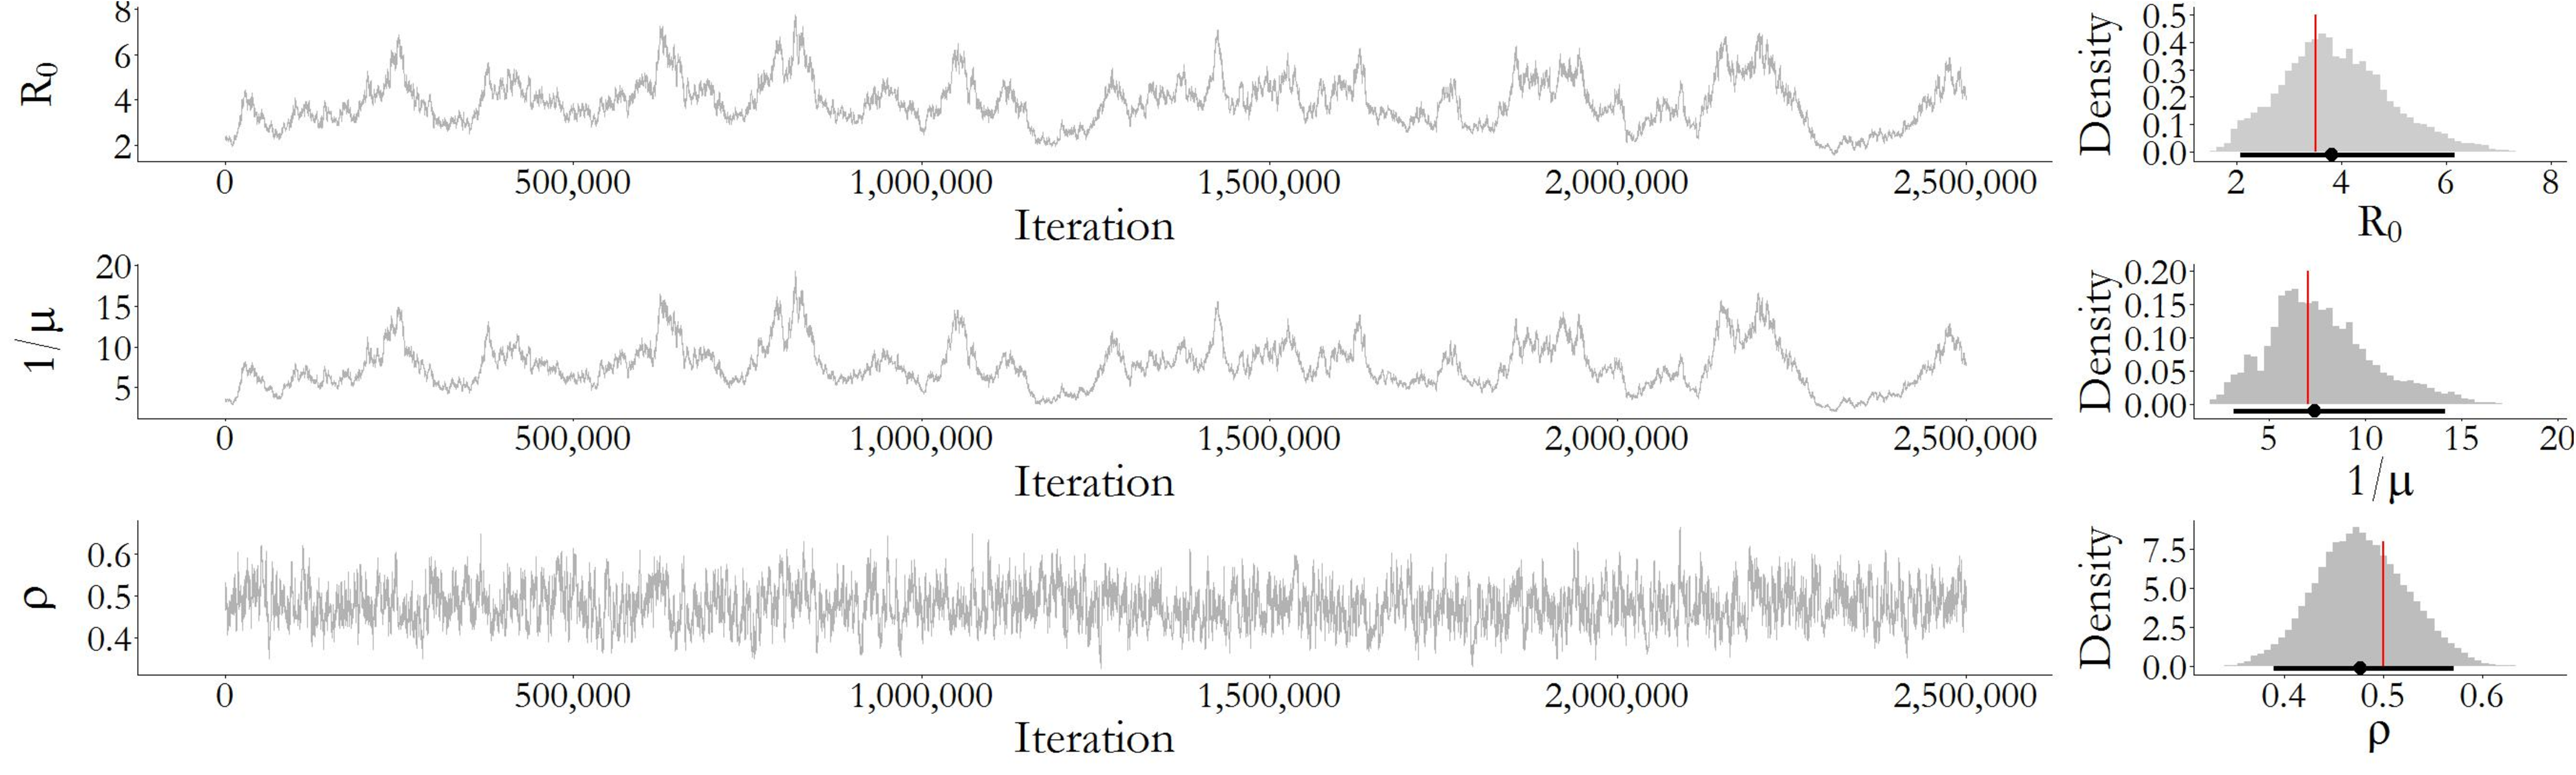
\includegraphics[width=0.9\textwidth]{figures/lna_centered_traces}
\caption{Posterior traceplots for parameters of interest sampled by a single MCMC chain of an SIR model fit to negative binomial distributed incidence data. MCMC targeted the posterior, \ref{eqn:lna_approximate_posterior}, alternately updating the non--restarting LNA for $ \bNtil|\btheta,\bY $ via elliptical slice sampling, and $ \btheta|\bNtil,\bY $ via a multivariate random walk Metropolis algorithm. $ R_0 = \beta N / \mu$ is the basic reproductive number, $ 1/\mu $ is the mean infectious period duration, and $ \rho $ is the mean case detection rate. The true values of $ R_0,\ 1/\mu,$ and $ \rho $ were 3.5, 7, and 0.5, respectively.}
\label{fig:lna_centered_traces}
\end{figure}

\subsubsection{Non--centered Parameterization}
\label{subsubsec:noncentered_parameterization}	

We can improve the mixing of our MCMC chains by reparameterizing the log--incidence process as a deterministic mapping of standard normal random variables, $ \bZ\sim MVN(\bs{0},\mb{I}) $, which are \textit{a priori} independent of the model parameters. This NCP is carried out by noting that if $ \bNtil(t_\ell)\sim MVN(\bmu(t\ell),\bSigma(t_\ell) $ and $ \bZ(t_\ell)\sim MVN(\bs{0},\mb{I}) $, then $ \bNtil \overset{\mcL}{=}\widetilde{\bW}(t_\ell),\ \widetilde{\bW}(t_\ell) = \bmu(t_\ell) + \bSigma(t_\ell)^{1/2}\bZ(t_\ell) $. We now target the joint posterior of the model parameters and the non--centered LNA draws,
\begin{align}
\label{eqn:lna_noncentered_posterior}
\pi(\btheta,\bZ|\bY) &\propto L(\bY|\doLNA(\bZ,\btheta,\mcI))\ind{\bN(\bZ,\btheta,\mcI)\in\mcS_N^R}\ind{\bX(\bZ,\btheta,\mcI)\in\mcS_X^R}\pi(\bZ)\pi(\btheta).
\end{align}
We will denote by $ \bN(\bZ,\btheta,\mcI) $ and $ \bX(\bZ,\btheta,\mcI) $ the incidence and prevalence sample paths that are output by the \doLNA\ procedure. The procedure for this mapping, denoted \doLNA, is presented in Algorithm (\ref{alg:doLNA}). 

\begin{algorithm}
	\caption{Mapping standard normal draws onto LNA sample paths.}
	\label{alg:doLNA}
	\begin{algorithmic}[1]
		\Procedure{doLNA}{$ \bZ,\btheta,\mcI $}
		\State \textbf{initialize: }$ \bX(t_0) \gets \bx_0,\ \bN(t_0) \gets \bs{0},\ \bNtil(t_0) \gets \bs{0},\ \bmu(t_0) \gets \bs{0},\ \bSigma(t_0) \gets \bs{0} $
		\For{$ \ell = 1,\dots,L $}
		\State $ \bmu(t_\ell),\ \bSigma(t_\ell) \gets $ solutions to (\ref{eqn:lna_ode_drift}) and (\ref{eqn:lna_ode_diffusion}) over $ (t_{\ell-1}, t_\ell] $
		\State $ \bNtil(t_\ell)\gets \bmu(t_\ell) + \bSigma(t_\ell)^{1/2}\bZ(t_\ell) $ \Comment{non--centered parameterization}
		\State $ \bN(t_\ell)\gets \bN(t_{\ell-1}) + \exp(\bNtil(t_\ell)) - \bs{1} $
		\State \textbf{restart initial conditions:} 
		\State {\hspace{0.2in} $ \bX(t_\ell) \gets \bX(t_{\ell-1}) + \bA^T(\bN(t_\ell)-\bN(t_{\ell-1})),\ \bNtil(t_\ell) \gets \bs{0},\ \bmu(t_\ell)\gets\bs{0},\ \bSigma(t_\ell)\gets\bs{0} $ }
		\EndFor
		\State \hspace{-0.25in}\Return \Comment{return incidence and/or prevalence sample paths}
		\State$\bN = \left \lbrace\bN(t_0),\bN(t_1),\dots,\bN(t_L)\right \rbrace,\ \bX = \left \lbrace \bX(t_0),\ \bX(t_1),\dots,\bX(t_\ell) \right \rbrace $
		\EndProcedure
	\end{algorithmic}
\end{algorithm}

The NCP of the log--incidence process substantially improves the mixing of MCMC chains that alternate between updates to $ \bZ|\btheta,\bY $ and $ \btheta|\bZ,\bY $. Figure \ref{fig:lna_centered_traces} shows traceplots of model parameters for one of MCMC chains for an SIR model fit to Poisson distributed incidence data using the centered parameterization (CP) of the LNA transition density. MCMC was run for 2.5 million iterations, following a tuning run of equal length, but each chain only manages to yield a effective sample sizes for $ R_0 $ and the infectious period duration in the low double digits. In contrast, the NCP yields effective sample sizes per--chain of between 500--700 for each of the model parameters in only 50,000 iterations, following a short tuning run of equal length. Figure \ref{fig:lna_noncentered_traces} shows the traceplot for one of the MCMC chains, which clearly mixes better. 

\begin{figure}[!ht]
	\centering
	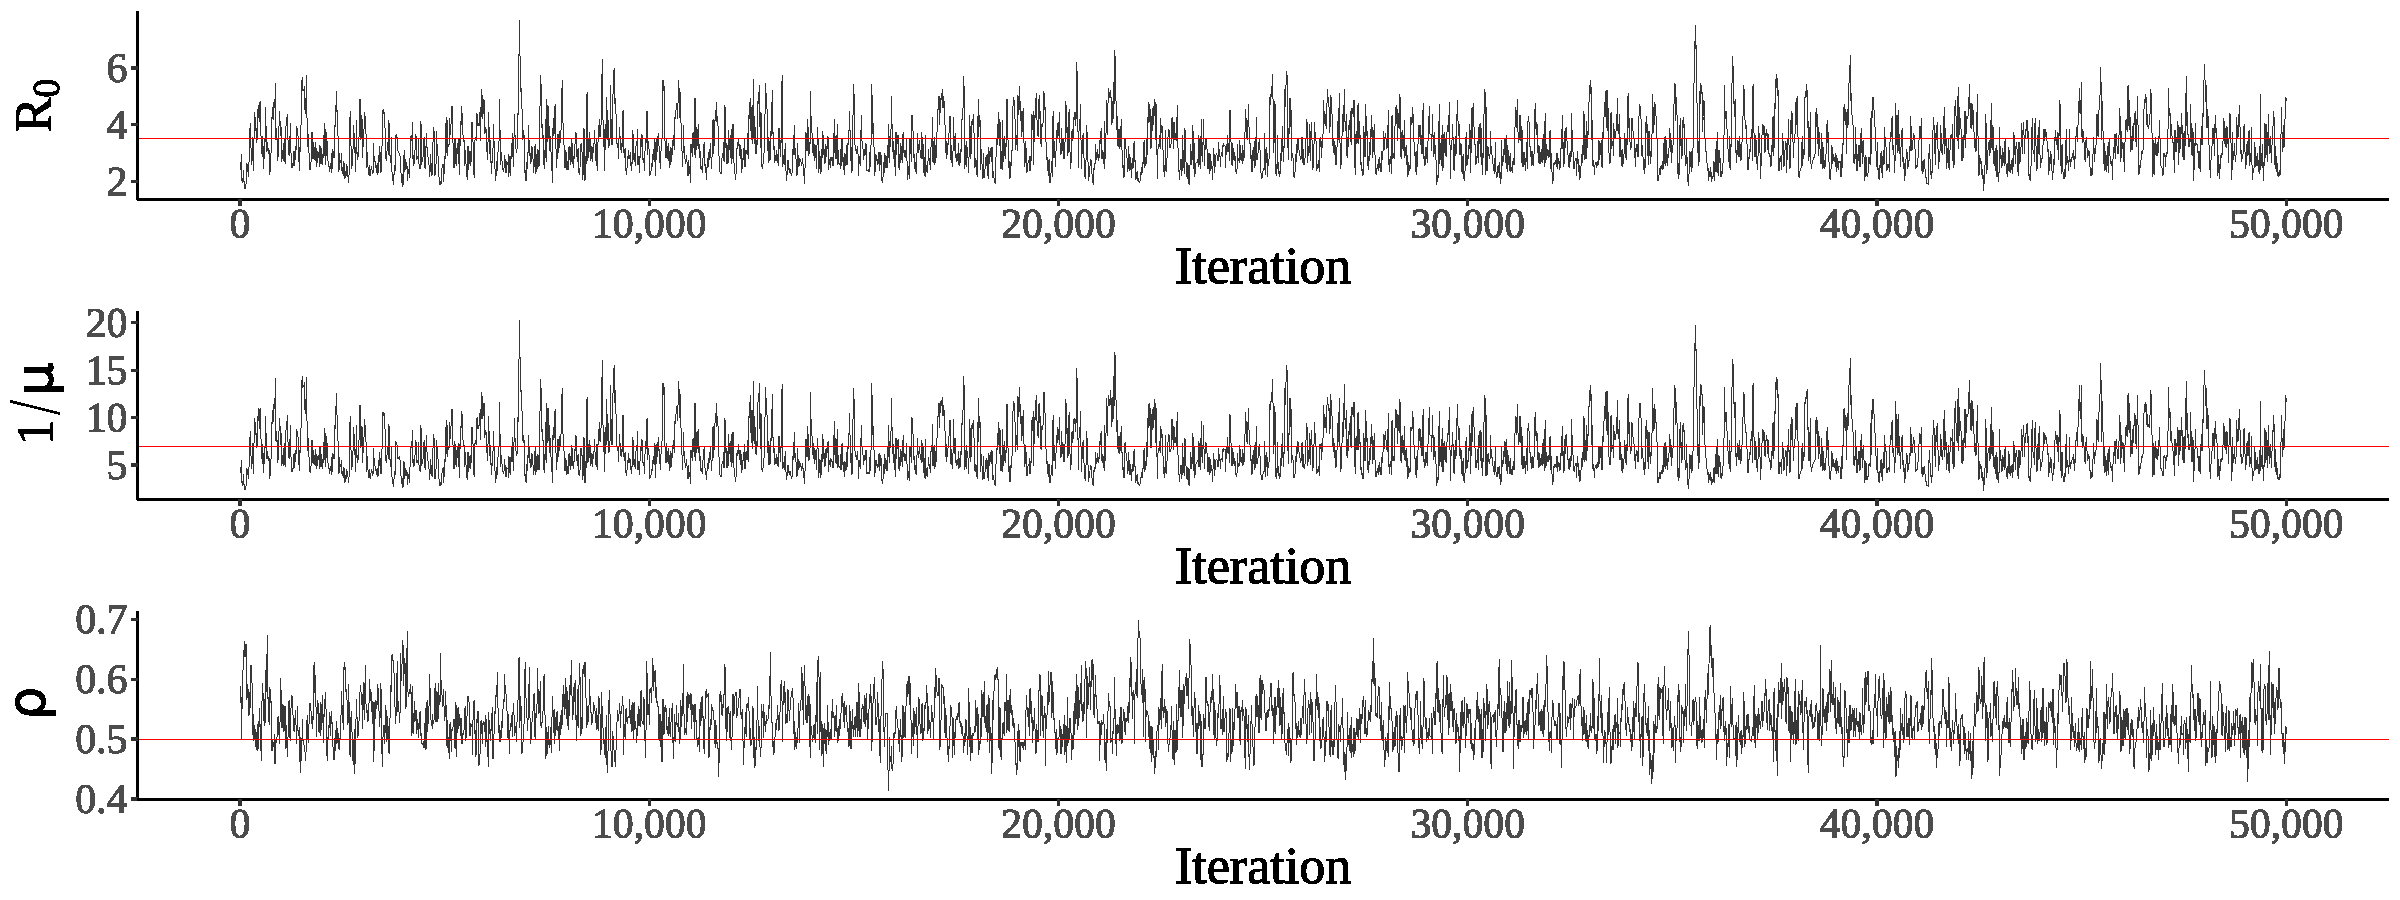
\includegraphics[width=0.9\textwidth]{figures/lna_noncentered_traces}
	\caption{Posterior traceplots for parameters of interest sampled by a single MCMC chain of an SIR model fit to Poisson distributed incidence data. MCMC targeted the posterior, \ref{eqn:lna_noncentered_posterior}, alternately updating $ \bZ|\btheta,\bY $ via elliptical slice sampling, and $ \btheta|\bZ,\bY $ via a multivariate random walk Metropolis algorithm. $ R_0 = \beta N / \mu$ is the basic reproductive number, $ 1/\mu $ is the mean infectious period duration, and $ \rho $ is the mean case detection rate. The true values of $ R_0,\ 1/\mu,$ and $ \rho $ were 3.5, 7, and 0.5, respectively.}
	\label{fig:lna_noncentered_traces}
\end{figure}

In each iteration of a DA MCMC algorithm, we alternate between updates to the latent path, conditional on the model parameters, and updates to the parameters, conditional on the latent path. Figure \ref{fig:lna_sampling_diagram}, which depicts the CP and NCP representations of an LNA path, provides some insight into why the NCP improves MCMC mixing. Under the CP (top plot), updates to $ \btheta|\bNtil,\bY $ are made conditionally on a \textit{fixed} LNA path. Therefore, proposed parameter values are accepted depending on whether they are concordant with the data \textit{and} the current path. Even small perturbations to model parameters can result in shifts of the LNA distributions (grey densities) that would render the current path (red points) unlikely under the proposal. In contrast, perturbations to parameters implicitly perturb an LNA path defined using the NCP, even as the LNA draws, $ \bZ $, are clamped to their current values. 

\begin{figure}[!ht]
	\centering
	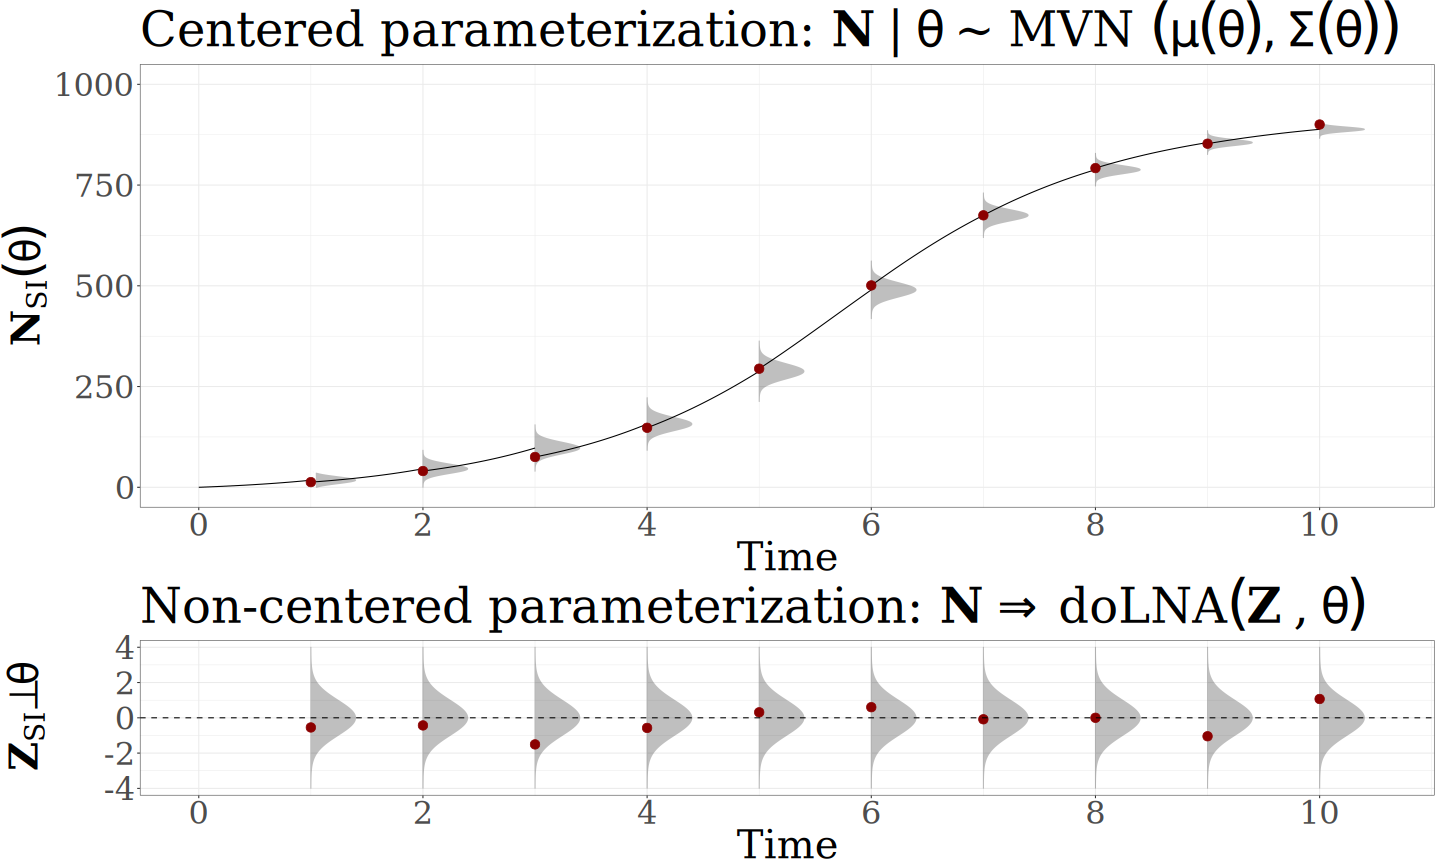
\includegraphics[width=0.9\textwidth]{figures/lna_sampling_diagram}
	\caption{Centered (top) and non--centered (bottom) parameterizations of an LNA incidence path. In the CP, the log--incidence is normally distributed with mean and covariance obtained by solving the LNA ODEs, (\ref{eqn:lna_ode_drift}) and (\ref{eqn:lna_ode_diffusion}). In the NCP, the log--incidence is a draw from a standard normal distribution that is deterministically mapped to a sample path via the $ \doLNA $ algorithm. In both the CP and NCP, state at the end of each interval determines the initial conditions of the LNA ODEs for the next interval. Plots of CP LNA transition densities are rescaled for clarity.}
	\label{fig:lna_sampling_diagram}
\end{figure}

The NCP of the LNA also plays an important role in facilitating efficient updates of $ \bZ|\btheta,\bY $ via the elliptical slice sampling (ElliptSS) algorithm of \cite{murray2010}, which was detailed in Section \ref{subsubsec:elliptical_slice_sampling} and is presented in Algorithm \ref{alg:elliptss_lna}. ElliptSS is an efficient and easy to implement MCMC algorithm for sampling Gaussian random variables, $ \bZ $, in models where the posterior of can be decomposed as the Gaussian prior for $ \bZ $ and an arbitrary likelihood, $ L(\bY|\bZ,\btheta) $, i.e.,
\begin{equation}
\label{eqn:eliptss_posterior_decomp}
\pi(\btheta,\bZ|\bY)\propto L(\bY|\bZ,\btheta)MVN(\bZ;\mu_\bZ,\bSigma_\bZ).
\end{equation}
The target posterior under the LNA NCP, (\ref{eqn:lna_noncentered_posterior}), is of this form, regardless of whether the LNA is restarted at the beginning of each inter--observation interval, as in \cite{fearnhead2014}, or the non--restarting version is used as in \cite{komorowski2009}. Note that the CP cannot be expressed as a jointly Gaussian collection of random variables with complete data likelihood of the form (\ref{eqn:eliptss_posterior_decomp}) when we use the restarting version of the LNA. Although each transition density, (\ref{eqn:lna_transition_density}), is itself Gaussian, the joint LNA path, $ \bN $, is not \textit{a priori} Gaussian when the LNA ODEs are restarted since the mean of $ \bN(t_\ell) $ depends non--linearly on the value of $ \bN(t_{\ell-1}) $. The quality of the LNA approximation is known to degenerate over long time intervals. Restarting the LNA ODEs has been established to improve the approximation when analyzing time series data of non--negligible length \cite{fearnhead2014,giagos2010inference}. Hence, use of the NCP is critical to enabling the use of ElliptSS for jointly updating of $ \bZ|\btheta,\bY $ when using the restarting version of the LNA. 

We note that the elliptical slice sampling Algorithm \ref{alg:elliptss_lna} differs slightly from the algorithm in \cite{murray2010} regarding how the initial proposal is made. In both cases, the distribution of proposed states, $ \bZ_{prop} $, is centered at the current state $ \bZ_{cur} $. However, the distribution of angles of accepted states using our algorithm will be centered around 0, whereas the distribution of angles for accepted proposals using the algorithm in \cite{murray2010} will be bimodal with peaks at 0 and $ 2\pi $. The algorithms are nevertheless equivalent due to the rotational symmetry of the proposals (a proposal made using an angle $ \phi $ is equivalent to a proposal using $ \phi+2\pi $). The original ElliptSS algorithm was modified for convenience since, in some cases, it will be advantageous to tune the initial ElliptSS bracket width to reduce the number of bracket contractions, and hence the number of likelihood evaluations requiring us to solve the LNA ODEs. This is discussed further in Section \ref{sec:lna_init_bracket_width}. When tuning the initial bracket width, we will typically set the initial width to a constant times the standard deviation of the angles that were accepted during some initial tuning run. Thus, it is easier if the distribution of accepted angles is symmetric about zero.

\begin{algorithm}[!ht]
	\caption{Sampling LNA draws via elliptical slice sampling.}
	\label{alg:elliptss_lna}
	\begin{algorithmic}[1]
		\Procedure{\doElliptSS}{$ \bZ_{cur},\btheta,\bY,\mcI,\omega = 2\pi $}
		\State Sample ellipse: $ \bZ_{prop} \sim N(\bs{0}, \mb{I}) $
		\State Sample threshold: $ u|\bx \sim \mr{Unif}(0, L(\bY|\doLNA(\bZ_{cur},\btheta,\mcI))) $
		\State Position the bracket and make initial proposal: \vspace{-0.1in}
		\begin{align*}
		\psi &\sim \mr{Unif}(0,\omega)\\
		L_\psi &\leftarrow -\psi;\ R_\psi \leftarrow L_\psi + \psi\\
		\phi &\sim \mr{Unif}(L_\psi,R_\psi)
		\end{align*}
		\State Set $ \bZ' \leftarrow \bZ_{cur}\cos(\phi) + \bZ_{prop}\sin(\phi) $. 
		\If{$ L(\bY|\doLNA(\bZ',\btheta,\mcI)) > u $}{ accept $ \bZ' $}
		\State\Return{ $ \bZ' $}
		\Else
		\State Shrink bracket and try a new angle.
		\State{\textbf{If:} $ \phi < 0 $}{ \textbf{then: }$ L_\phi \leftarrow\phi $ }{ \textbf{else: }$ R_\phi \leftarrow \phi $}
		\State $ \phi \sim \mr{Unif}(L_\phi, R_\phi) $.
		\State \textbf{GoTo:} 5.
		\EndIf
		\EndProcedure
	\end{algorithmic}
\end{algorithm}

\subsubsection{Initializing the LNA draws}
\label{subsubsec:lna_init}
In simple models, reasonable parameter values will generally lead to valid LNA paths for initial $ \bZ\sim MVN(\bs{0},\mb{I}) $, i.e., paths that satisfy the monotonicity and positivity conditions, and thus have non--zero likelihood. However, this is not necessarily the case for complex models with many types of transition events, or when the time--series of incidence counts is long. One option is to include a re--sampling step after line 6 in Algorithm \ref{alg:doLNA}, in which $ \bZ(t_\ell) $ is redrawn in place until the conditions for a valid path over the interval are met. It is important to note that such a procedure does not sample from the correct distribution since $ \bZ $ is not actually a truncated multivariate Gaussian. To correct for this, we will ``warm--up" the LNA path with an initial run of $ \doElliptSS $ iterations in which the likelihood only consists of the indicators for whether the path is valid. Finally, note that ElliptSS, or any valid MCMC algorithm for updating $ \bZ|\btheta,\bY $ for that matter, will never lead to an invalid LNA path being accepted if the current LNA draws and model parameters correspond to a valid path. Similarly, updates to model parameters conditional on the LNA draws will also preserve the validity of LNA paths.

\subsubsection{Parameter updates}
\label{subsubsec:lna_param_updates}
Each MCMC iteration will consist of a number of ElliptSS updates, typically one but possibly 2--3 for complex models, followed by a set of parameter updates. We will generally use either a global adaptive random walk Metropolis algorithm (Algorithm 4 in \cite{andrieu2008tutorial}) or the adaptive non--isotropic Gaussian slice sampler (GSS) presented in Section \ref{subsubsec:slice_sampling}. In models where the initial state, $ \bX_0 $, is not fixed, we will assign the prior $ \bX_0 \sim TMVN_{\mcS_X^R}\left (N\mb{p}, N(\diag(\mb{p}) - \mb{p}\mb{p}^T)\right ) $, which is a truncated multivariate normal approximation to a multinomial with initial state probabilities, $ \mb{p} $, constrained to the state space of compartment volumes. We update $ \bX_0 $ jointly with the LNA path via ElliptSS. Additional details are presented in Section \ref{sec:lna_init_volumes}.

We have found it helpful, for the purpose of assigning sensible priors to model parameters and for improving MCMC mixing and convergence, to parameterize the estimation scale on which the MCMC explores the parameter space in terms of how the parameters directly affect the model dynamics. For the SIR model, this might mean re-expressing the model parameters in terms of the basic reproductive number of an outbreak, $ R0 = \beta N /\mu $, and the recovery rate, $ \mu $. Additionally, we would like our estimation scale to be unconstrained and therefore sample (and either accept or reject) values for $ \log(R0) $ and $ \log(\mu) $. The importance of appropriately parameterizing the estimation scale is discussed further in Section \ref{sec:est_scale_discussion}. 

\subsection{Assessing model fit}
\label{subsec:lna_model_diags}

\subsection{Implementation}
\label{subsec:lna_implementation}
The algorithms for approximate inference via the LNA and ODE models are implemented in the \texttt{stemr} $ \R $ package, which can be available, along with vignettes, from the following stable GitHub repository: \texttt{https://github.com/fintzij/stemr}. The implementation is flexible and provides facilities for specification of arbitrary SEM dynamics, a variety of emission probability distributions, and capabilities for accommodating time--varying covariates, time--varying parameters, and deterministic forcings. Computationally intensive operations are implemented in C++ via \texttt{Rcpp} and \texttt{RcppArmadillo} \cite{rcpp,rcpparmadillo}. ODE integration functions are dynamically compiled in \texttt{C++} with the help of the \texttt{odeintr} R package \cite{odeintr} and ODEs can be integrated using a variety of methods available in the \texttt{Odeint} library \cite{ahnert2011odeint}. Additional aspects of the implementation are discussed in Section \ref{sec:lna_implementation_vignettes}

\section{Simulations}
\label{sec:lna_simulations}

\subsection{Motivating Use of the LNA --- Comparison with Common SEM Approximations}
\label{subsec:lna_coverage}

The LNA is by no means the only approximation of the transition density of the MJP representation of a SEM. In the following subsection, we will illustrate why the LNA is an attractive choice, balancing computational cost with fidelity of the MJP approximation. We benchmark the LNA against two commonly used approximations of the MJP: the deterministic approximation given by a system of deterministic ODEs that are the functional infinite population limit of the MJP \cite{fuchs2013inference}, and a discrete--time approximation of the MJP using a multinomial modification of the $ \tau $--leaping algorithm (MMTL) \cite{breto2011compound} to simulate epidemic paths within a particle marginal Metropolis--Hastings (PMMH) framework \cite{andrieu2010particle}. The ODE approximation was chosen because of its ubiquity in the study of epidemic modeling, while the MMTL approximation in combination with PMMH was chosen because of a straightforward and general implementation in the popular \texttt{pomp} package in \texttt{R} \cite{pompjss}. Arguably, the MMTL approximation is somewhat closer to the original MJP than the LNA since it preserves the discreteness of the latent state space, while the ODE approximation, being deterministic, is \textit{a priori} further removed from the MJP.

The fidelity of each approximation to the original MJP depends on the population size and the epidemic dynamics. Outbreaks with explosive dynamics in large populations will tend to deviate less, relatively, from their infinite population deterministic limits than outbreaks that occur in small populations, that are less contagious, or that are characterized by uncertainty in the probability and timing of a major outbreak. We fit SIR models to 500 datasets simulated under a range of SIR dynamics. Each dataset is simulated by drawing the model parameters from a set of prior distributions, simulating an outbreak via Gillespie's direct algorithm \cite{gillespie1976general}, and finally simulating the dataset as a negative binomial sample of the true incidence. Datasets arising from outbreaks that died off immediately were discarded and re--simulated, while datasets arising from outbreaks lasting longer than 50 epochs were truncated at 50 observations. SIR models were then fit via the LNA, ODE, and MMTL approximations under the priors used in the data generating process. The simulation was repeated under three different regimes for the population size and the initial number of infected individuals, reflecting different levels of inherent stochasticity in the epidemic behavior and chosen because they reflect typical population sizes in which the three methods might be applied without being so large that the MJP path would be essentially deterministic. All individuals who were not initially infected were susceptible at the start of each outbreak (i.e., no individuals with pre-existing immunity). The population sizes, initial conditions, and priors are given in Table \ref{tab:lna_coverage_sim}. The population size and initial conditions for each run were assumed to be known. Therefore, the only model misspecification was in the approximation used for the latent epidemic process. Additional results and details about the simulation setup are provided in Section \ref{sec:lna_coverage_supplement}. We also performed four analogous supplementary simulations, with similar results, where we generated datasets under fixed parameter regimes (presented in Section \ref{sec:lna_fixedpar_coverage}).

\begin{table}[!ht]
	\label{tab:lna_coverage_sim}
	\caption{Population sizes, initial conditions, and priors under which datasets were simulated. Five hundred datasets were simulated for each of the population size regimesEach outbreak was simulated from a MJP with SIR dynamics. The observed incidence was a negative binomial sample of the true incidence in each inter--observation interval.}\small
	\centering
	\begin{tabular}{lccc}
		
		& \textbf{Regime 1} & \textbf{Regime 2} & \textbf{Regime 3} \\\hline
		\textbf{Population size ($ N $)} & 10,000 & 50,000 & 250,000 \\ 
		\textbf{Initial infecteds ($ I_0 $)} & 1 & 5 & 25 \\
		\hline
		&&&
	\end{tabular} 

	\begin{tabular}{cllc}
		\textbf{Parameter} & \textbf{Interpretation} & \textbf{Prior} & \textbf{Median (95\% Interval)} \\ \hline
		$ R0-1 $ & Basic reproduction \# - 1 & LogNormal(0, 0.25) & $ \implies R0 = $ 2.00 (1.38, 3.66) \\ 
		$ 1/\mu $ & Mean infectious period & LogNormal(0.7, 0.13)& 2.01 (1.01, 4.00) \\
		$ \rho / (1-\rho) $ & Odds of case detection & LogNormal(0, 1) & $ \implies \rho =$ 0.5 (0.12, 0.88) \\
		$ \phi $ & Neg.Binom. overdispersion & Exponential(0.1) & 6.93 (0.25, 36.89)\\
		\hline
	\end{tabular}
\end{table}

\subsubsection{Results}

This simulation was designed to be generous to the approximations that were used in fitting SEMs to the simulated data. The initial compartment counts and true population sizes were known, and there was no misspecification with respect to either the sampling model or the epidemic dynamics. Despite this, the ODE models struggle to reliably recover the true parameters, particularly those governing the sampling process. As shown in Figure \ref{fig:lna_coverage_main}, coverage of credible intervals for ODE models was low for all model parameters, and this was only somewhat mitigated as the population size increased. Coverage of credible intervals for models fit via the LNA and via MMTL was close to the nominal 95\% level for all model parameters in all three population size regimes. Further inspection of the posterior median errors (middle row of Figure \ref{fig:lna_coverage_main}) and the widths of 95\% credible intervals (bottom row of Figure \ref{fig:lna_coverage_main}) provides intuition for why the ODE performs so poorly. Estimates of the case detection probability tend to be high and estimates of the negative binomial over--dispersion parameter are low (corresponding to large variances in the conditional distribution of observed incidence). Furthermore, credible intervals for the basic reproductive number and recovery rate obtained via the ODE approximation tend to be narrower than LNA and MMTL credible intervals. This is in agreement with findings by other authors who have found that ODE models tend to underestimate uncertainty in epidemic dynamics (see e.g., \cite{king2015avoidable}). Taken together, these results suggest that the LNA is, at least in this simple example, about as good at approximating the original MJP as is the more exact MMTL. 

\begin{figure}[!ht]
	\centering
	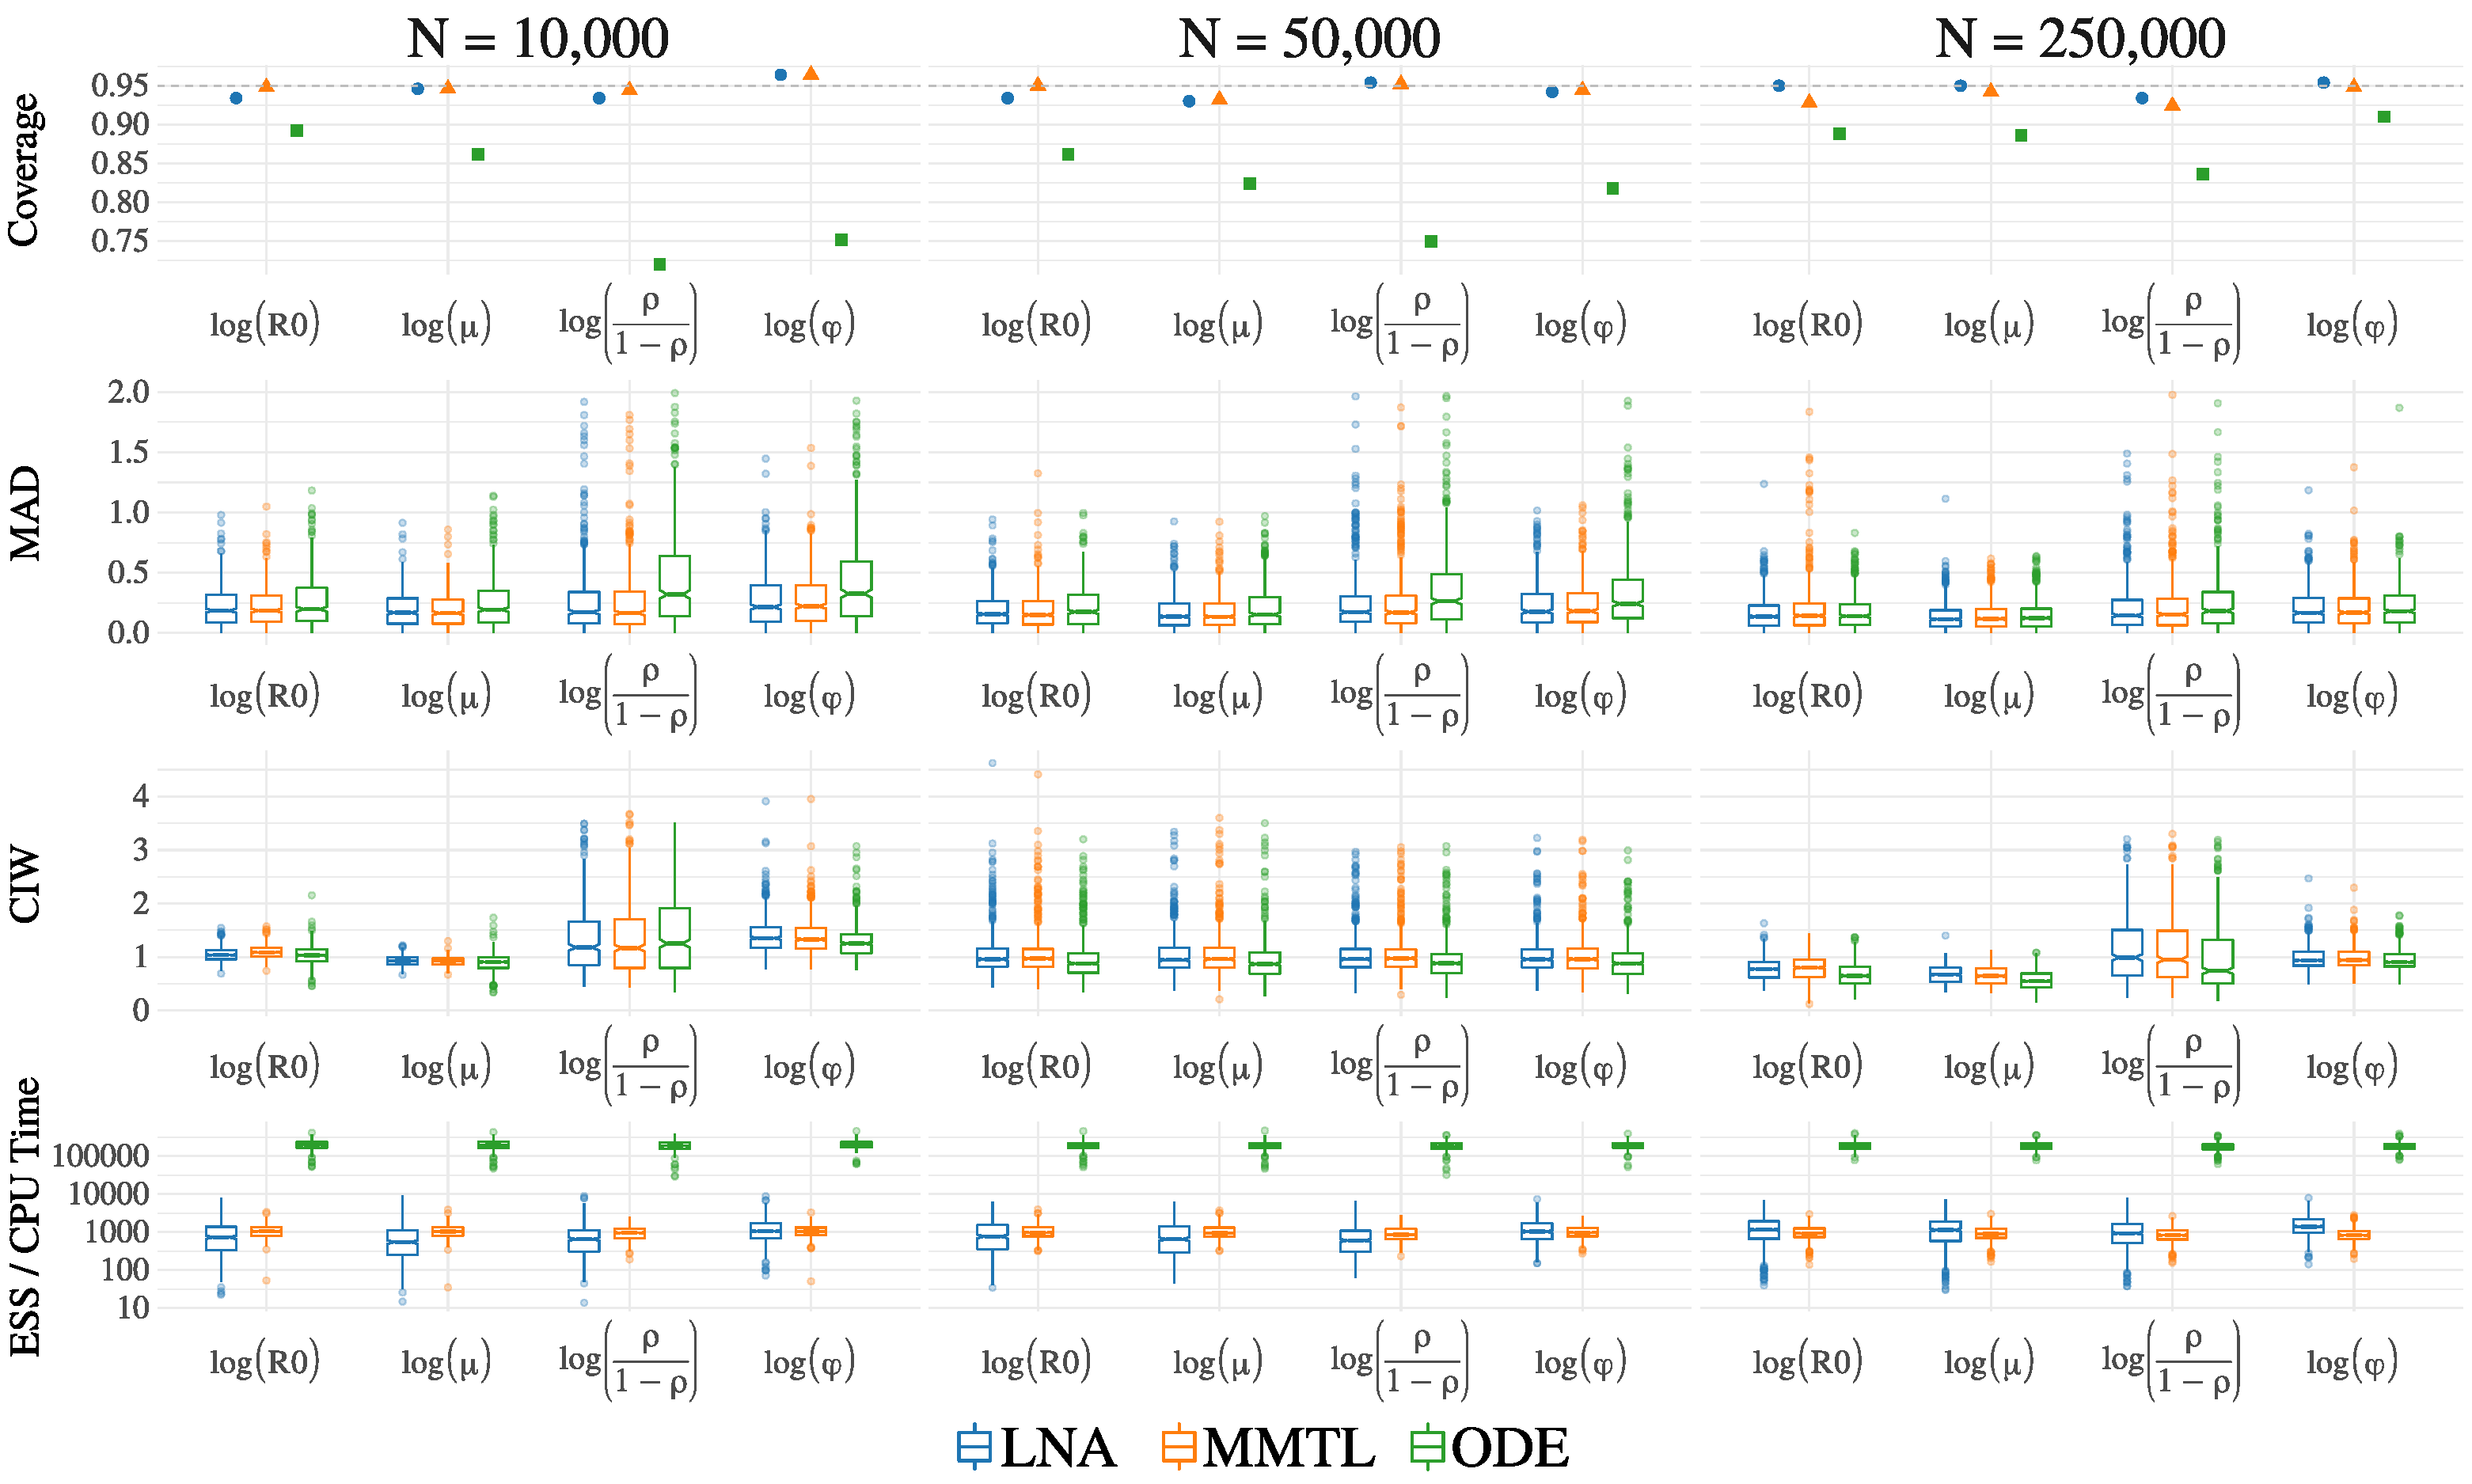
\includegraphics[width=\textwidth]{figures/lna_coverage_plots_main}
	\caption{Comparison of results from SIR models fit to 500 datasets simulated in populations of three different sizes. Models were fit via the linear noise approximation (LNA), multinomial modified $ \tau $--leaping (MMTL) within particle marginal Metropolis--Hastings, and deterministic ordinary differential equations (ODE). Summary statistics were computed for meaningful functionals of model parameters. $ R_0 $ is the basic reproductive number of an outbreak, $ \mu $ is the recovery rate, $ \rho $ is the negative binomial case detection probability, $ \phi $ is the negative binomial over--dispersion parameter. From the top, the rows correspond to the proportion of runs where the 95\% Bayesian credible interval covered the true parameter values, the differences between the posterior medians and the true values, and the widths of 95\% Bayesian credible intervals. The simulation was repeated for three population sizes and initial numbers of infected individuals (columns).}
	\label{fig:lna_coverage_main}
\end{figure}

We note that these results are not intended to suggest that there is no place for ODE models in the computational toolbox of disease modelers. To the contrary, when time is of the essence, as in an outbreak setting, crude estimates via the ODE may be obtained quickly. Average ODE run times were substantially shorter than LNA and MMTL run times and required far less CPU time per effective sample (see Table \ref{tab:lna_coverage_compstats}). ODE models are also appealing because they lend themselves to analytic characterizations of various aspects of the outbreak dynamics, e.g., relating the final outbreak size to the basic reproductive number (see, e.g., \cite{andersson2000stochastic,britton2018,keeling2008}).

 In this simple simulation, the LNA and MMTL approximations had comparable computational performance, with the LNA perhaps being somewhat faster, but also with the caveat that comparing the ODE/LNA approximations with the MMTL approximation on the basis of computational performance is a bit misleading since the comparison would have turned out differently had we made other choices for the LNA and MCMC settings (e.g., timestep of MMTL, number of particles in PMMH, or tuning the initial EllipSS bracket width for the LNA). The important point to make regarding computational performance is that as model dynamics get more complex and the time series get longer, approximations, such as MMTL, that are used within a particle filter framework, such as PMMH, will become computationally infeasible. In many cases, the lack of an adequate model from which to simulate particle paths will lead to issues of particle degeneracy and an inability to fit even simple models (see \cite{fintzi2017efficient} for an example). Indeed, PMMH was abandoned as a computational strategy for analyzing Ebola data in later sections because of difficulty fitting SEMs with reasonable effort. However, as we shall see in the following sections, the LNA remains performant even as the model dynamics increase in complexity. 
 
 \begin{table}[!h]
 	\label{tab:lna_coverage_compstats}
 	\caption{Run times, effective sample sizes, and relative geometric mean (GM) log--posterior effective sample size (ESS) per CPU time for models fit via the ODE, LNA, and MMTL approximations. Run times and ESS are computed over all chains. The GM log--posterior ESS/CPU time was computed over the five chains for each model and divided by the corresponding GM ESS/CPU time for the MMTL model. We report 50\% (2.5\%, 97.5\%) quantiles of the CPU time, ESS, and relative GM ESS/CPU time.}\footnotesize
 	\centering
 	\begin{tabular}{lccc}		
 		& \textbf{ODE} & \textbf{LNA} & \textbf{MMTL} \\\hline
 		CPU time (minutes) &  0.42 (0.23, 0.64) & 27.78  (12.03, 56.25) & 86.96 (40.47, 159.68) \\ 
 		Effective sample size & 5745 (4557, 6616) & 4067   (346, 11313) & 6834 (3764, 11879) \\
 		GM ESS/CPU time vs. MMTL & 180 (90, 350) & 1.87 (0.14, 8.84) & --- \\
 		\hline
 		&&&
 	\end{tabular} 
 \end{table}
